% Chapter Template

\chapter{Introduction} % Main chapter title

\label{Chapter1} % Change X to a consecutive number; for referencing this chapter elsewhere, use \ref{ChapterX}

%----------------------------------------------------------------------------------------
%	SECTION 1
%----------------------------------------------------------------------------------------

This introductory chapter provides an overview of the thesis goals and the basic background behind the method reasoning. 
The following sections present: (\ref{sec1}) the reason for the secure smartphone project; (\ref{sec2}) an introduction to the MEGA65 project; and (\ref{sec3}) the scope, research questions and design requirements of the project. 
This chapter concludes with a brief outline of the remainder of this thesis.

\section{Computer Security has become a Shared Delusion}
\label{sec1}

The last few years has seen a disturbing upward trend in the number and severity of security vulnerabilities in modern computing devices.
Whereas traditionally these security vulnerabilities have existed primarily in software, the ever-growing complexity of computer hardware, and in particular CPU designs, now means that we are beginning to see many more hardware-based vulnerabilities.
Indeed, the complexity of the {\em errata} for a modern processor is now often longer\cite{6thGener70:online} than the entire specification of early generation processors \cite{mos6500m32:online}.
Whereas software vulnerabilities can be quickly and economically patched, this is not always the case for hardware-based vulnerabilities, as it may require replacement of the defective hardware\cite{WillHuge39:online}.  
It also means that when a fix is issued, that there will likely be hundreds of millions of devices that remain incurably vulnerable for the remainder of their lives \cite{Intellef1:online}.

        Modern computers are designed to achieve increasing performance and functionality through the easiest route.
        This is typically done by adding in extra layers of logic, consequently increasing sophistication and complicating the system.
        The processors of these modern computers are optimised using speculative execution, which is a technique used by high-speed processors in order to increase performance by guessing future likely execution paths \cite{RN16}.
        This complexity however can be detrimental to security, because it becomes increasingly difficult and expensive to verify the correct operation of these more complicated devices.
        This is not merely a theoretical problem: There have been a number of recent cases where vulnerabilities have been exploited, in specific the Spectre and Meltdown hardware attacks, and the Via C3 ''God mode'' bit \cite{ViaC3x865:online}.

        The recent Spectre \cite{RN16} and Meltdown \cite{RN3} vulnerabilities are headline examples of this trend and the difficulties that such vulnerabilities create.
        Intel and the other vendors are still struggling to produce patches that do not reduce the reliability or performance of their processors, while mitigating as much of the threat posed by these vulnerabilities as possible \cite{Ifatfirs66:online}.
        At the end of the day, the only fully effective solution is for them to develop a new generation of processors that have the defects corrected in the silicon – an extremely expensive and time-consuming process.
        Even then, it is likely that the performance of those processors will be lower, precisely because it is performance optimisations that are the direct cause of the vulnerabilities.
        Even if processors are created that correct these known issues, they too could be found to suffer from one or more hitherto unknown vulnerabilities, and themselves require replacement.
        When commerce, personal privacy and security as well as national security depends on the correct and secure operation of computers, we clearly have a problem of considerable importance before us.

        It is precisely this problem of the impossibility of feasibly verifying the security of complex modern devices that is the reason for this project, and it's reconsideration of the merits of simpler, albeit less performant architectures.
The overall project aim is to create a secure smartphone based on a purposely simple architecture, that is capable of basic telephony functions and simple productivity tasks.
Where a trade-off must be made between security and richness of functions, the trade-offs will usually tend towards security.


The system’s architecture will be based on the Commodore 64 computer, to ensure that the device not only simple enough to be secure, but to ensure that it can be sufficiently productive.
In this context, the existing productivity software, tools and developer base and knowledge to be leveraged, and also exist as a kind of proof-by-example that the resulting system will have sufficient functionality to be useful for a variety of tasks.


\section{Designing a secure 8-bit smart-phone}
\label{sec2}

The MEGA65 project is an existing project within the Telecommunications Research Laboratory to build a Commodore 64 compatible computer, which is described in more detail in the literature review.
Its original goal was to produce and open-source reproduction of the commercially unreleased Commodore 65 (C65) \cite{MEGA65MO64:online}.
Further, work has already commenced to create a portable version of the MEGA65, complete with touch-screen interface.
Thus it represents a system with a simple architecture and with full source code availability, which can be used within this thesis as the basis for the creation of a simple and secure communications device.

This thesis will therefore explore the adaption of the MEGA65 retro-computer to produce a simple and secure communications device, focusing
on the hardware requirements, definition and realisation.
One of the key issues to be resolved is how the untrustably complex cellular network interface module, i.e., the cellular modem, of a smart-phone can be segregated and managed, so that the security of the whole device is not compromised.
Thus one area of focus will be how to design a device that restricts the cellular modem, and for particularly sensitive activities allows it to be deprived of power.

More specifically, we posit that to create such a device that is both secure and usable, that:
\begin{itemize}
	\item It must be able to power down the FPGA used to implement the system when idling on the cellular network, so that power consumption is similar to a conventional cellular phone.\\
	\item It must be able to power down any untrustable components such as the cellular modem, both under software control, and via physical switches under the control of the user of the device. This present special challenges because the cellular modem is able to draw 4A, and thus a relatively large electronic switch is required.\\
\end{itemize}

%-----------------------------------
%	SECTION 3
%-----------------------------------

\section{Research Questions \& Scope}
\label{sec3}

The recognition of the preceeding facts and situations leads this thesis to consider the following research questions:
\begin{enumerate}
	\item \textit{What are the core use cases and functional requirements required to create a useful and secure communications device?}\\
	\item \textit{How can those functional requirements be translated into the design for a secure communications device that is feasible to be manufactured in a University research environment?}\\
	\item \textit{Given the necessity to include a complex cellular modem in the design, how can that device be contained, and when necessary deprived of power?}\\
	\item \textit{How can the complex power management requirements of this device be met?}\\
	\item \textit{What trade-offs, if any, are required to satisfy the functional and dimensional requirements of the MEGA65 phone PCB, within the financial and time constraints of this project?}\\
\end{enumerate}

%-----------------------------------
%	SECTION 3
%-----------------------------------
\section{Structure of Thesis}

Following this chapter, Chapter \ref{Chapter2} provides background information on the project, including an indepth study on the insecurity of modern complex CPUs.\\ 
Chapter \ref{Chapter3} follows this with a list of required use cases of the secure phone, accompanied with a use story for each use case.
The functional requirements derived from each use case has then been compiled into one functional requirements list.\\ 
In Chapter \ref{Chapter3} a list of hardware requirements is derived from the list of functional requirements.\\
Chapter \ref{Chapter5} gives an overview of the component selection and circuit design. 
This includes the method and selection process behind all the major components as well as the method and ideology behind all the circuit designs.\\
Chapter \ref{Chapter6} describes the schematic layout from the circuit design, moving into the PCB layout from the schematic design.
This section details errors and challenges found during the schematic design process, as well as the method behind the PCB layout and any errors and challenges found during the PCB layout stage.\\
Chapter \ref{Chapter7} provides the discussion of the project, which details the major implemention challenges of both the schematic and PCB stages, and answers the research questions based on the results of the project.\\
Finally, the conclusion of the project is provided in Chapter \ref{Chapter8}.
This summarises the project's goals and results, draws conclusions, and closes the dissertation with suggestions for further research.\\
The following block diagram (Figure \ref{fig:methodology}) displays the design process of the project, with the four major sections coloured accordingly. The start of each major section includes this diagram with the accompanying section coloured in. 

\begin{figure}
	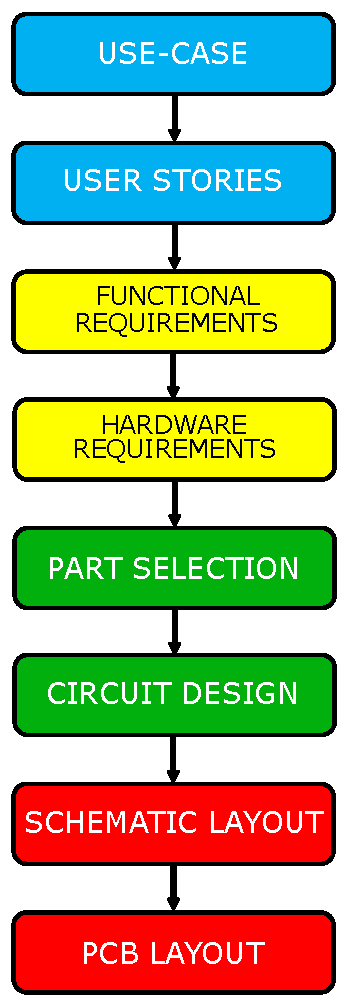
\includegraphics[width=0.5\linewidth]{Figures/first_table.pdf}\centering
	\caption{Design Process}
	\label{fig:methodology}
\end{figure}
